\documentclass[a4paper]{slides}
%\usepackage[koi8-r]{inputenc}
%\usepackage{russianb}
\usepackage[pdftex,landscape]{geometry}
\usepackage{amsmath,amsthm,amssymb,lscape}
\usepackage{graphicx}
\pagestyle{empty}
\tolerance 1000
\topmargin -5cm
\textheight=25cm
\textwidth=27cm
\hoffset=-3cm
\newcommand {\W}{W_1^1}
\newcommand {\Wf}{\stackrel{o\ }{W_1^1}}
\newcommand{\Real}{\mathbb R}
\renewcommand {\bar}[1]{\overline{#1}}
\renewcommand {\ge}{\geqslant}
\renewcommand {\le}{\leqslant}
\newcommand{\abs}[1]{\left\vert#1\right\vert}
\relpenalty=10000

\begin{document}

\begin{slide}
\large
Step 1 --- sketch of the proof.
\begin{center}
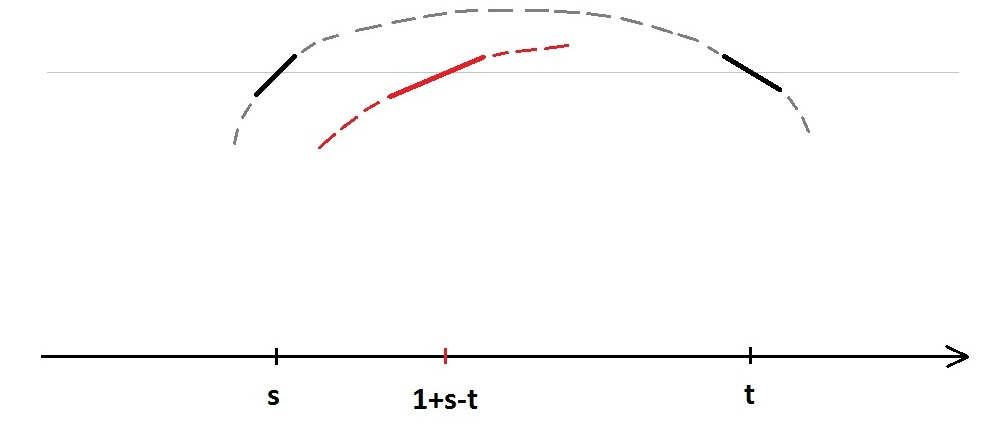
\includegraphics[width=250mm]{level1}
\end{center}

$a(1 + s + t) \le a(s) + a(t) \Leftrightarrow a(1 + s - t) \le a(s) + a(t)$

$\abs{\bar{u}'(1 + s - t)} \le \min\left\{\abs{u'(s)}, \abs{u'(t)}\right\} \Rightarrow I(\bar{u}) \le I(u)$

\end{slide}
\end{document}
